
\(P(t) = 100t\e^{-t}\).

\subsection*{1.}

\[
P(0) = 100 \times 0 \times \e^0 = 0 \quad \text{et} \quad P(5) = 100 \times 5 \times \e^{-5} \approx 3.
\]

\subsection*{2.}

\(P'(t) = 100(1 - t)\e^{-t}\).

\paragraph{a.} On sait que, quel que soit le réel \(t\), \(\e^{-t} > 0\) et par conséquent \(100\e^{-t} > 0\). Le signe de \(P'(t)\) est donc celui de \(1 - t\) qui est positif sur \([0 \,;\, 1]\) et négatif sur \([1 \,;\, 5]\).

\paragraph{b.} La fonction \(P\) est donc croissante sur \([0 \,;\, 1]\) puis décroissante sur \([1 \,;\, 5]\), avec un maximum en :
\[
P(1) = 100\e^{-1} \approx 36{,}78.
\]

\begin{center}
\begin{tikzpicture}
\tkzTabInit[lgt=3.5, espcl=4]{$x$ / 1, {Signe de $f'(x)$} / 1, {$f(x)$} / 2}{${0}$, ${1}$, ${5}$}
\tkzTabLine{,+,0,-,}
\tkzTabVar{-/{$0$},+/{$100\e^{-1} \approx 36{,}78$},-/{$500\e^{-5} \approx 3$}}{/}
\end{tikzpicture}
\end{center}

\paragraph{c.} D'après la question précédente et comme le confirme la courbe représentative de la fonction, \(P(1) \approx 36{,}78\) est le maximum de la fonction sur l'intervalle \([0 \,;\, 5]\).

\subsection*{3.}

On constate graphiquement qu'après 4 h 30 min, \(P(t) < 5\). Le polluant ne sera plus dangereux après 4 h 30 min.

